\section{\IIC Protokol} \label{sec:I2C_protokol}
Dette afsnit omhandler kommunikationen mellem alle \IIC kommunikerende komponenter i projektet.

\subsection{Temp-/Luftfugtighedssensor}
Information om Temperatur- og Luftfugtighedssensor er fundet under komponentens datasheet. Bilag 004 \cite{lib:TempHum_I2C}.

%Slave Temp-/Luftfugtihed
\begin{table}[h]
\centering
\begin{tabularx}{0.6\textwidth}{| X | X |} 			\hline
\textbf{Slave:} 		& Temp-/Luftfugtighed		\\ \hline
\textbf{Adresse:}		& 0x27						\\ \hline
\textbf{Bemærkninger:}	& scl: 100-400 kHz			\\ \hline
\end{tabularx}
\caption{\IIC Oplysninger for Temp-/Luftfugtigedhedssensor}
\label{tbl:I2CTempLuftOplysninger}
\end{table}


Når der skal læses data fra sensoren, sker det jf. Figur \ref{fig:I2CTempLuftProtokol}, fundet under Bilag 004 side 2 \cite{lib:TempHum_I2C}.


\begin{figure}[h]
\centering
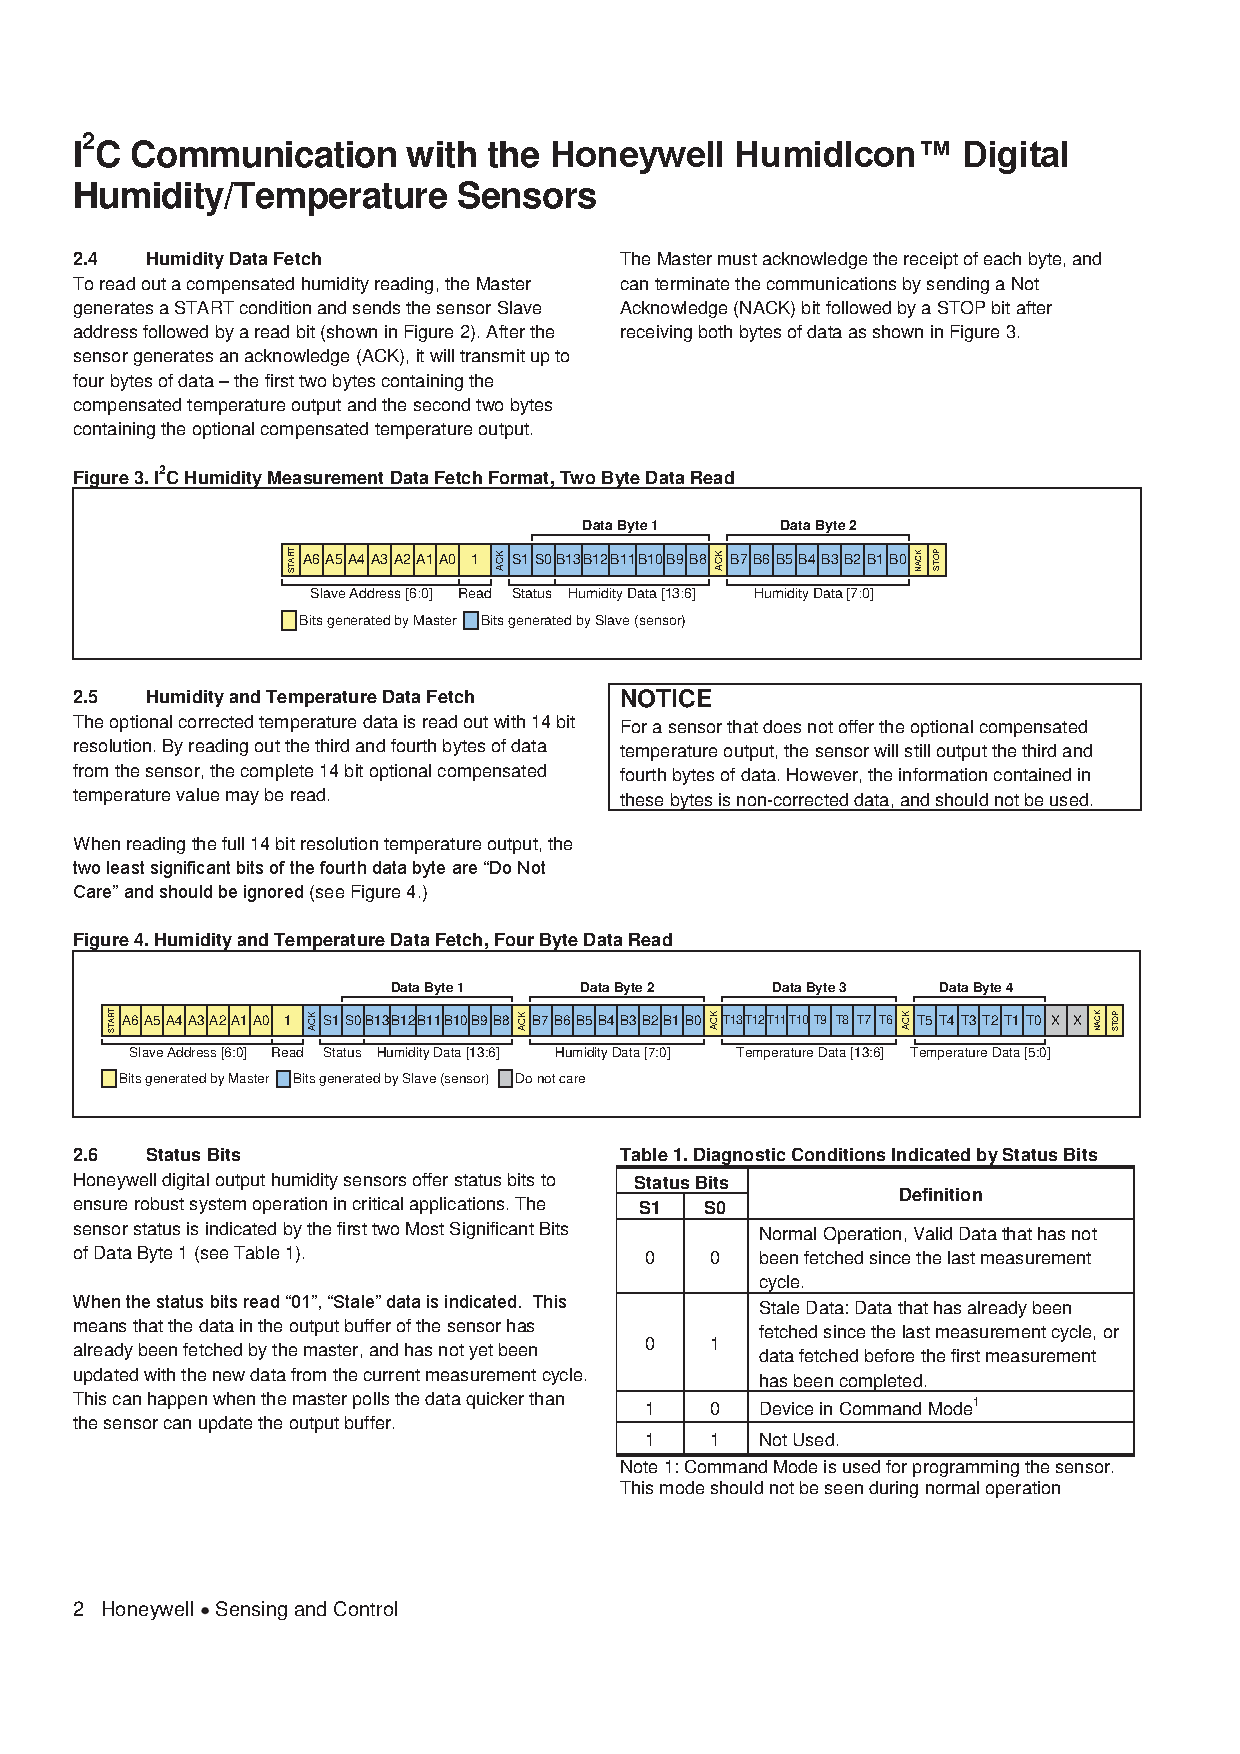
\includegraphics[width=\textwidth - 1 cm, clip=true, trim=48 319 55 471]{../fig/I2CTempLuftProtokol.pdf}
\caption{\IIC protokol for Temp-/Luftfugtighedssensor}
\label{fig:I2CTempLuftProtokol}
\end{figure}

\clearpage

\subsection{Slave Aktuator}
%Slave Aktuator
\begin{table}[h]
\centering
\begin{tabularx}{0.6\textwidth}{| X | X |} 			\hline
\multicolumn{2}{ | l | }{\textbf{Adresse:} 0x42} 	\\ \hline
\textbf{Kommando} 		& \textbf{Beskrivelse}		\\ \hline
WriteAdjustWindow		& Åbning/Lukning af vindue	\\ \hline
WriteAdjustHeat			& Tænd/Sluk for varme		\\ \hline
WriteAdjustVentilation	& Juster ventilation		\\ \hline
WriteAdjustIrrigation	& Juster vanding			\\ \hline
ReadStatus				& Anmodning om status		\\ \hline
\end{tabularx}
\caption{\IIC Kommandoer for Slave Aktuator}
\label{tbl:I2CAktuatorKommandoer}
\end{table}



%WriteAdjustWindow
\begin{table}[h]
\centering
\begin{tabularx}{0.6\textwidth}{| >{\centering\arraybackslash}X | >{\centering\arraybackslash}X | >{\centering\arraybackslash}X | >{\centering\arraybackslash}X | >{\centering\arraybackslash}X | >{\centering\arraybackslash}X | >{\centering\arraybackslash}X | >{\centering\arraybackslash}X |}	\hline
W7 & W6 & W5 & W4 & W3 & W2 & W1 & W0				\\ \hline
\multicolumn{2}{ | l | }{0x0} 						&
\multicolumn{2}{  l | }{Don't Cares}				&
\multicolumn{4}{  l | }{Position for vindue,}
\\
\multicolumn{2}{ | l | }{} 							&
\multicolumn{2}{  l | }{}							&
\multicolumn{4}{  l | }{0x0 = lukket, 0xF = åben}
\\ \hline
\end{tabularx}
\caption{\IIC Kommando WriteAdjustWindow}
\label{tbl:I2CAktuatorKommandoWriteAdjustWindow}
\end{table}



%WriteAdjustHeat
\begin{table}[h]
\centering
\begin{tabularx}{0.6\textwidth}{| >{\centering\arraybackslash}X | >{\centering\arraybackslash}X | >{\centering\arraybackslash}X | >{\centering\arraybackslash}X | >{\centering\arraybackslash}X | >{\centering\arraybackslash}X | >{\centering\arraybackslash}X | >{\centering\arraybackslash}X |}	\hline
H7 & H6 & H5 & H4 & H3 & H2 & H1 & H0				\\ \hline
\multicolumn{2}{ | l | }{0x1} 						&
\multicolumn{3}{  l | }{Don't Care}					&
\multicolumn{3}{  l | }{Tænd/Sluk}
\\
\multicolumn{2}{ | l | }{} 							&
\multicolumn{3}{  l | }{}							&
\multicolumn{3}{  l | }{varmelegeme,}
\\
\multicolumn{2}{ | l | }{} 							&
\multicolumn{3}{  l | }{}							&
\multicolumn{3}{  l | }{0x0 = off, 0x7 = on}
\\ \hline
\end{tabularx}
\caption{\IIC Kommando WriteAdjustHeat}
\label{tbl:I2CAktuatorKommandoWriteAdjustHeat}
\end{table}

\clearpage

%WriteAdjustVentilation
\begin{table}[h]
\centering
\begin{tabularx}{0.6\textwidth}{| >{\centering\arraybackslash}X | >{\centering\arraybackslash}X | >{\centering\arraybackslash}X | >{\centering\arraybackslash}X | >{\centering\arraybackslash}X | >{\centering\arraybackslash}X | >{\centering\arraybackslash}X | >{\centering\arraybackslash}X |}	\hline
V7 & V6 & V5 & V4 & V3 & V2 & V1 & V0				\\ \hline
\multicolumn{2}{ | l | }{0x2} 						&
\multicolumn{3}{  l | }{Don't Care}					&
\multicolumn{3}{  l | }{Tænd/Sluk}
\\
\multicolumn{2}{ | l | }{} 							&
\multicolumn{3}{  l | }{}							&
\multicolumn{3}{  l | }{ventilation,}
\\
\multicolumn{2}{ | l | }{} 							&
\multicolumn{3}{  l | }{}							&
\multicolumn{3}{  l | }{0x0 = off, 0x7 = on}
\\ \hline
\end{tabularx}
\caption{\IIC Kommando WriteAdjustVentilation}
\label{tbl:I2CAktuatorKommandoWriteAdjustVentilation}
\end{table}



%WriteAdjustIrrigation
\begin{table}[h]
\centering
\begin{tabularx}{0.6\textwidth}{| >{\centering\arraybackslash}X | >{\centering\arraybackslash}X | >{\centering\arraybackslash}X | >{\centering\arraybackslash}X | >{\centering\arraybackslash}X | >{\centering\arraybackslash}X | >{\centering\arraybackslash}X | >{\centering\arraybackslash}X |}	\hline
I7 & I6 & I5 & I4 & I3 & I2 & I1 & I0				\\ \hline
\multicolumn{2}{ | l | }{0x3} 						&
\multicolumn{6}{  l | }{Værdi for pins til vanding,}
\\
\multicolumn{2}{ | l | }{} 							&
\multicolumn{6}{  l | }{I5: nr. 6 – I0: nr. 1,}
\\
\multicolumn{2}{ | l | }{} 							&
\multicolumn{6}{  l | }{1 = on, 0 = off}
\\ \hline
\end{tabularx}
\caption{\IIC Kommando WriteAdjustIrrigation}
\label{tbl:I2CAktuatorKommandoWriteAdjustIrrigation}
\end{table}



%ReadStatus
\begin{table}[!h]
\begin{tabularx}{\textwidth}{| >{\centering\arraybackslash}X | >{\centering\arraybackslash}X | >{\centering\arraybackslash}X | >{\centering\arraybackslash}X | >{\centering\arraybackslash}X | >{\centering\arraybackslash}X | >{\centering\arraybackslash}X | >{\centering\arraybackslash}X | >{\centering\arraybackslash}X | >{\centering\arraybackslash}X | >{\centering\arraybackslash}X | >{\centering\arraybackslash}X | >{\centering\arraybackslash}X | >{\centering\arraybackslash}X | >{\centering\arraybackslash}X | >{\centering\arraybackslash}X |}	\hline
W3 & W2 & W1 & W0 & H2 & H1 & H0 & V2 & V1 & V0 & I5 & I4 & I3 & I2 & I1 & I0				\\ \hline
\multicolumn{4}{ | l | }{Position for vindue,} 			&
\multicolumn{3}{  l | }{Status for}						&
\multicolumn{3}{  l | }{Status for}						&
\multicolumn{6}{  l | }{Status for pins til vanding,}
\\
\multicolumn{4}{ | l | }{0x0 = lukket,} 				&
\multicolumn{3}{  l | }{Varmelegeme,}					&
\multicolumn{3}{  l | }{ventilation,}					&
\multicolumn{6}{  l | }{I5: nr. 6 – I0: nr. 1,}	
\\
\multicolumn{4}{ | l | }{0xF = åben} 					&
\multicolumn{3}{  l | }{1 = on,}						&
\multicolumn{3}{  l | }{0x0 = off,}						&
\multicolumn{6}{  l | }{1 = on,}
\\
\multicolumn{4}{ | l | }{} 								&
\multicolumn{3}{  l | }{0 = off}						&
\multicolumn{3}{  l | }{0x7 = on}						&
\multicolumn{6}{  l | }{0 = off}					
\\ \hline
\end{tabularx}
\caption{\IIC Kommando ReadStatus}
\label{tbl:I2CAktuatorKommandoReadStatus}
\end{table}

\clearpage